\documentclass{llncs}
%%%%%%%%%%%%%%%%%%%%%%%%%%%%%%%%%%%%%%%%%%%%%%%%%%%%%%%%%%%%%%%%%%%%%%%%%%%%%%%%
% Lattice-native BFV sigma protocol (v4) with per-share NIZK verification
% LatticeFold+ lattice-native folding (sole backend); Track A (Nova BN254+Grumpkin) removed June 2026
% committed-smudge decryption; G2 full in-circuit Poseidon commitment verification
% Real UltraHonk Solidity verifier (N=65536, 28 G1 points)
% Research prototype — do not use for The Interfold or any production deployment
%%%%%%%%%%%%%%%%%%%%%%%%%%%%%%%%%%%%%%%%%%%%%%%%%%%%%%%%%%%%%%%%%%%%%%%%%%%%%%%%
% Paper strategy: UNIFIED (see .sisyphus/design/p2/paper-strategy-decision.md, C.D.5 APPROVE)
% Target venue: Crypto 2027 (primary), Eurocrypt 2027 (fallback), CCS 2026 (fast-track)

\usepackage[utf8]{inputenc}
\usepackage{amsmath,amssymb,amsfonts}
\usepackage{hyperref}
\usepackage{amsthm}

\newtheorem{theorem}{Theorem}[section]
\newtheorem{lemma}[theorem]{Lemma}
\newtheorem{definition}[theorem]{Definition}

\title{PVTHFHE: Private-Verifiable Threshold Fully Homomorphic Encryption}
\author{Anonymous Authors}
\institute{Under Submission}

\begin{document}

\maketitle

\begin{abstract}
We present PVTHFHE, a research prototype for private-verifiable threshold fully homomorphic encryption
targeting $O(n)$ per-party work and $O(\text{polylog}\, n)$ verifier cost.
Our construction combines a PVSS-based distributed key generation (P4), a lattice NIZK
well-formedness argument (P1), a LatticeFold+ accumulation scheme over RLWE (P2), and an
EVM on-chain verifier surrogate (P3). We prove correctness, soundness, and zero-knowledge for the core sub-protocols and validate the implementation via end-to-end benchmarks, noting where cryptographic surrogates are used.
\end{abstract}

\section{Introduction}

Threshold fully homomorphic encryption (ThFHE) enables a set of $n$ parties to jointly evaluate
circuits on encrypted data without any single party holding the full secret key. When combined
with publicly verifiable proofs, each computation step becomes auditable by any observer.

Our main contribution is a unified four-layer protocol (P4 $\to$ P1 $\to$ P2 $\to$ P3) that
targets $O(n)$ per-party work during the setup phase and $O(\text{polylog}\, n)$ on-chain
verification cost.

The current prototype implements: a lattice-native BFV sigma protocol (\texttt{bfv\_sigma.rs},
533 loc) proving BFV encryption correctness over RNS with binary challenges and masking bound
$2^{30}$; committed-smudge decryption via \texttt{partial\_decrypt\_committed\_smudge}; a
single canonical DKG path with \texttt{FoldTrackKind::Sk} and \texttt{FoldTrackKind::ESm} share domains;
proof format version~4 (\texttt{PROOF\_VERSION = 4}) with per-share NIZK verification;
\texttt{verify\_shares} enabled in the demo path (no longer compiled out); D.2 batched
share-encryption proof covering sk+esm domains with independent commitments via
\texttt{batch\_verify\_share\_encryption}; D.3 per-domain separation preventing
cross-domain replay (domain tags in \texttt{pvthfhe-domain-tags}); E.1/E.2 pipeline verifier
wiring for batched Shamir share-computation and DKG aggregation relations; F.2 smudge-slot
freshness enforcement via public \texttt{SlotRegistry} rejecting slot reuse.
P2 uses LatticeFold+ lattice-native folding over RLWE as the sole folding backend.

\section{Related Work}

Prior work on threshold FHE includes \cite{boneh2010threshold}. Lattice-based NIZK arguments
are studied in \cite{lyubashevsky2012lattice}. LatticeFold was introduced in
\cite{latticefold2024}. Our P3 on-chain verifier builds on EVM proof verification techniques
from \cite{groth16evm}.

\section{Preliminaries}

Let $R = \mathbb{Z}[X]/(X^n + 1)$ be the cyclotomic ring with $R_q = R/qR$.
We assume the Module Learning With Errors (MLWE) and Module Short Integer Solution (MSIS)
problems are hard. All protocols operate in the Random Oracle Model (ROM).

\section{P4: PVSS Key Generation}
\label{sec:p4}

The P4 sub-protocol implements a publicly-verifiable secret sharing (PVSS) distributed key
generation. Each party $i$ contributes a Shamir share $s_i$ over $\mathbb{F}_{2^{61}-1}$,
and the dealer's commitment is verified via SHA-256.

\begin{theorem}[P4 Correctness]
\label{thm:p4-t1}
An accepted honest keygen transcript yields the unique serialized \texttt{BFVPublicKey}
placeholder reconstructed from the dealer's Shamir secret over $2^{61}-1$.
\end{theorem}
\begin{proof}
By inspection of the commitment scheme and the Shamir reconstruction over $\mathbb{F}_{2^{61}-1}$;
see \texttt{docs/security-proofs/p4/t1-correctness.md} for the full argument.
\end{proof}

\begin{theorem}[P4 Static Secrecy]
\label{thm:p4-t2}
Any static adversary corrupting fewer than $t$ parties learns no additional information about
the Shamir-shared secret under the current simulation; real Ring-LWE secrecy is deferred.
\end{theorem}
\begin{proof}
The simulator constructs an indistinguishable view by sampling fresh shares for corrupted
parties; see \texttt{docs/security-proofs/p4/t2-secrecy.md}.
\end{proof}

\begin{theorem}[P4 Public Verifiability Soundness]
\label{thm:p4-t3}
Any artifact accepted by \texttt{verify\_transcript}, together with transcript shares passing
public replay, corresponds to a valid SHA-256-commitment-consistent dealing.
\end{theorem}
\begin{proof}
Follows from SHA-256 collision resistance; see \texttt{docs/security-proofs/p4/t3-public-verifiability-soundness.md}.
\end{proof}

\begin{theorem}[P4 Abort-with-Blame Robustness]
\label{thm:p4-t4}
Misbehavior covered by the implemented commitment-recomputation predicates yields
publicly checkable blame against the cheater, while honest parties are never falsely blamed.
\end{theorem}
\begin{proof}
Proved by case analysis over the concrete blame predicates defined in \texttt{docs/security-proofs/p4/t4-abort-with-blame-robustness.md}.
\end{proof}

\begin{theorem}[P4 Sequential Composition]
\label{thm:p4-t5}
The simulated P4 session/public-key handoff composes sequentially with the P1
decrypt-share functionality at the exported interface boundary.
\end{theorem}

\section{P1: Lattice NIZK}
\label{sec:p1}

The P1 sub-protocol consists of two sigma-proof components. The first is a SLAP-style
sigma protocol for RLWE well-formedness, compiled via Fiat--Shamir. The second is a
lattice-native BFV encryption-correctness proof (\texttt{bfv\_sigma.rs}) that proves,
per CRT limb over the RNS decomposition, knowledge of bounded $(m, \mathbf{u}, e_0, e_1)$
satisfying $\mathsf{ct}_0 = \mathsf{pk}_0 \cdot \mathbf{u} + e_0 + \Delta \cdot m$
and $\mathsf{ct}_1 = \mathsf{pk}_1 \cdot \mathbf{u} + e_1$. It uses binary challenges
$\{0,1\}^N$, a masking bound of $2^{30}$, and RNS-accelerated verification. Masking
seeds were upgraded from deterministic to \texttt{OsRng} in Round~1 remediation.
Together these two sub-protocols provide witness-free lattice proofs of well-formedness
for RLWE ciphertexts.

\begin{theorem}[P1 Completeness]
\label{thm:p1-t1}
Honest witnesses satisfying the implemented SHA-256 commitment opening, bounded-error check,
and SLAP-style transcript equations always yield an accepting P1 proof.
\end{theorem}

\begin{theorem}[P1 Knowledge Soundness]
\label{thm:p1-t2}
Any accepting P1 prover yields a rewinding extractor (ROM, forking lemma) recovering the opened witness for the
implemented relation, except with probability bounded by the SHA-256 binding failure probability.
\end{theorem}

\begin{theorem}[P1 Zero-Knowledge]
\label{thm:p1-t3}
The serialized ShareNizkProof format achieves computational ZK — masked sigma transcript only, no witness openings. Fresh OsRng masks per invocation. VERDICT: APPROVE for full serialized format.
\end{theorem}


\begin{theorem}[P1 Simulation-Extractability Deferred]
\label{thm:p1-t4}
Simulation-extractability is not part of the frozen P1 baseline because P2 does not consume
simulated accepting P1 transcripts; a stronger theorem is required only if that interface
changes.
\end{theorem}

\begin{theorem}[P1 Commitment Binding]
\label{thm:p1-t5}
\texttt{pvss\_commitment} is binding on domain $\mathrm{SHA256}(\mathit{session\_id} \;\|\;
\mathit{participant\_id\_le} \;\|\; \mathit{secret\_share\_be})$ under SHA-256 collision resistance.
\end{theorem}

\section{P2: LatticeFold+ over RLWE}
\label{sec:p2}

The P2 sub-protocol accumulates P1 proofs, reducing on-chain verification
cost from $O(n)$ to $O(\text{polylog}\, n)$.  PVTHFHE uses
LatticeFold+ over RLWE as its sole folding backend.  P4 (PVSS key
generation, \S\ref{sec:p4}) and P1 (lattice NIZK, \S\ref{sec:p1}) provide
the front-end.

An earlier prototype used Sonobe Nova IVC over BN254/Grumpkin; this was
replaced by LatticeFold+ (now~\S\ref{sec:p2}) in June~2026.

The Cyclo crate (\texttt{pvthfhe-cyclo}) provides:
\texttt{fold\_one\_deterministic}, \texttt{verify\_fold},
\texttt{check\_satisfiability} (real CCS relation $M \cdot z \odot z = 0$
over BN254 $\mathbb{F}_r$), Ajtai lattice commitments ($Q_{\text{commit}} =
2^{49}$, 13~ring elements $\times$ 256~coeffs), and Fiat-Shamir challenge
derivation (\texttt{challenge\_v2} with \texttt{params\_digest} binding).
All 15~Cyclo tests pass including forgery resistance.

A heterogeneous IVC prototype (MicroNova compressor with
LatticeFoldTreeCircuitFamily) is available via
\texttt{PVTHFHE\_COMPRESSOR=micronova}. See
\texttt{ARCHITECTURE.md} \S MicroNova for details.

The implemented P2 path uses \textbf{LatticeFold+} accumulation that folds
RLWE ciphertext witnesses directly via algebraic relations, with a CCS
encoding of the Cyclo decryption relation~\cite{cyclo2025,latticefold2024}.

\begin{theorem}[P2-T1: LatticeFold+ Folding Completeness]
\label{thm:p2-t1}
Honest Cyclo-folded RLWE witnesses produce valid LatticeFold+ accumulator
instances satisfying the frozen verifier equation over the ternary challenge
space $\{-1,0,1\}$.
\textbf{Status: ASPIRATIONAL} (proof sketch only; contingent on
LatticeFold+ instantiation at frozen parameters).
\end{theorem}

\begin{theorem}[P2-T2: LatticeFold+ Knowledge Soundness]
\label{thm:p2-t2}
A depth-$d$ LatticeFold+ fold tree yields valid RLWE witnesses except
with $(1/3)^d$ plus SHA-256 binding failure probability.
\textbf{Status: CONTINGENT on Lemma~9 (Conjecture)}.
The formal reduction depends on the Cyclo joint knowledge extractor
(Lemma~9, \texttt{docs/security-proofs/lemma9.md}), which remains
unproven.  See implementation plan \texttt{p2-latticefold-target.md}.
\end{theorem}

\begin{theorem}[P2-T3: LatticeFold+ ZK Preservation]
\label{thm:p2-t3}
The LatticeFold+ scheme preserves the projected SLAP core zero-knowledge
view under ROM + HVZK assumptions, with additive $d \cdot (\varepsilon_{\text{HVZK}} +
\varepsilon_{\text{SHA-256}})$ distinguishing advantage.
\textbf{Status: ASPIRATIONAL} (proof sketch under
LatticeFold+ folding rules; no known blocker).
\end{theorem}

\begin{theorem}[P2-T4: LatticeFold+ Accumulator Binding]
\label{thm:p2-t4}
When instantiated as a linear lattice commitment
$\mathsf{Com}_{\mathbf{A}}(\mathbf{w}) = \mathbf{A} \cdot \mathbf{w} \bmod q$
with norm enforcement $\|\mathbf{w}\|_\infty \leq 17$, the LatticeFold+
accumulator is binding under RingSIS/M-SIS at $q = 65537$, $N = 1024$,
$\beta = 34$.
\textbf{Status: ASPIRATIONAL} (reduction is standard; blocked on norm enforcement
implementation per \texttt{docs/security-proofs/p2/T4.md}).
\end{theorem}

\begin{theorem}[P2-T5: LatticeFold+ On-chain Compatibility]
\label{thm:p2-t5}
The LatticeFold+ accumulator targets on-chain UltraHonk verification
($\approx 39{,}687$~gas) via the P3 path (\S\ref{sec:p3}).
\textbf{Status: ASPIRATIONAL} (projected from MicroNova gas estimates;
not yet implemented).
\end{theorem}

\textbf{Dependency note.}  All theorems above P2-T2 are blocked
on Lemma~9 (Conjecture) in \texttt{docs/security-proofs/lemma9.md}.  The
implementation roadmap is defined in
\texttt{.sisyphus/plans/p2-latticefold-target.md}.

\section{P3: On-Chain Verifier}
\label{sec:p3}

The P3 on-chain verifier is a Solidity contract that accepts the
accumulated P2 proof and finalizes the protocol on Ethereum.
PVTHFHE targets UltraHonk on-chain verification of the LatticeFold+
terminal accumulator.

\textbf{Current status.}  A real UltraHonk proof
(7{,}776 bytes, N=65{,}536, LOG\_N=16) from the Noir
\texttt{aggregator\_final} circuit was verified on Foundry at
1{,}885{,}528~gas using a generated \texttt{HonkVerifier.sol} (2{,}220
lines).  VK generation uses \texttt{bb write\_vk --oracle\_hash keccak}
for EVM-compatible 1{,}888-byte VKs.  A post-processing script
(\texttt{split-honk-vk.py}) rewrites the single massive struct literal
into sequential assignments to avoid EVM stack overflow (116~G1 points).
Sepolia deploy pending.  See \texttt{contracts/test/HonkVerifierRealProof.t.sol}
for the gas measurement.

\subsection{UltraHonk + MicroNova On-Chain Verification}
\label{sec:p3-ultrahonk}

The P3 path replaces the former trusted-signer surrogate with a
full on-chain cryptographic verifier for the LatticeFold+ terminal
accumulator (P2 output).  The projected stack is:

\begin{enumerate}
\item \textbf{MicroNova} compresses the LatticeFold+ recursive fold
  tree into a single constant-size proof over the BN254/Grumpkin cycle;
\item \textbf{UltraHonk} verifies the MicroNova proof on-chain via
  EIP-196/197 BN254 pairing precompiles, consuming a projected
  $39{,}687$~gas.
\end{enumerate}

\begin{theorem}[P3-T1: UltraHonk Verifier Soundness]
\label{thm:p3-t1}
On-chain UltraHonk acceptance implies a valid LatticeFold+ terminal
accumulator satisfying the frozen P2 verifier relation.
\textbf{Status: SKELETON} (\texttt{docs/security-proofs/p3/proof-skeletons.md}).
Dependent on MicroNova compression soundness and UltraHonk knowledge
soundness over BN254.
\end{theorem}

\begin{theorem}[P3-T2: Wrap Preserves Soundness]
\label{thm:p3-t2}
The MicroNova $\to$ UltraHonk compression preserves the LatticeFold+
accumulator soundness without lossy projection.
\textbf{Status: SKELETON}.
\end{theorem}

\begin{theorem}[P3-T3: Trusted-Setup Analysis]
\label{thm:p3-t3}
UltraHonk requires no trusted setup; MicroNova may require an SRS
(dependent on final UltraHonk variant).
\textbf{Status: SKELETON}.
\end{theorem}

\begin{theorem}[P3-T4: Gas Bound]
\label{thm:p3-t4}
Projected UltraHonk gas: $39{,}687$ (MicroNova 2-party compressed;
source: \texttt{.sisyphus/research/p3/prior-art.md}).
\textbf{Status: SKELETON} (projection, not yet measured on deployed contract).
\end{theorem}

\begin{theorem}[P3-T5: Liveness \& Blame]
\label{thm:p3-t5}
Abort-with-public-blame predicates extend to the UltraHonk verifier
with proof-invalid detection at the BN254
pairing-check level.
\textbf{Status: SKELETON}.
\end{theorem}

\textbf{Dependency note.}  All P3 theorems are skeletons pending:
(a) MicroNova integration with LatticeFold+ terminal proofs, and
(b) UltraHonk verifier contract deployment.  Implementation roadmap in
\texttt{.sisyphus/plans/p3-micronova-target.md}.

\textbf{Open problem P4 (on-chain IVC verification).}  Full on-chain
LatticeFold+ IVC verification remains an open problem.  The current
UltraHonk path verifies a wrapped MicroNova proof; direct on-chain
verification of the LatticeFold+ accumulator is projected for future
work.

\section{Security Analysis}

The security of the full PVTHFHE protocol follows by sequential composition (Theorem~\ref{thm:p4-t5})
from the security of its sub-protocols. The complete argument is structured as:
P4 correctness + secrecy $\Rightarrow$ P1 inputs are well-formed $\Rightarrow$ P2 accumulation
is sound $\Rightarrow$ P3 on-chain acceptance is valid.

\subsection{Threshold Decryption and CPAD Resistance}

Standard IND-CPA security is insufficient for threshold FHE because partial decryption
shares $d_i = c_1 \cdot sk_i + e_{\text{smudge},i}$ leak information about secret key
shares $sk_i$, effectively providing a decryption oracle. Checri et
al.\ \cite{checri2024cpad} showed that chosen-plaintext attacks with decryption
(IND-CPAD) are practical, recovering keys in under one hour on commodity hardware
against TFHE-rs, OpenFHE, and Lattigo.

PVTHFHE counters CPAD through \emph{noise flooding} as formalized by Boudgoust et
al.\ \cite{boudgoust2023threshold}: each partial decryption share is additively masked
with a fresh Gaussian noise polynomial $e_{\text{smudge}} \sim \mathcal{D}_{\mathbb{Z},
\sigma_{\text{smudge}}}$ with standard deviation $\sigma_{\text{smudge}} = 2^{40}
\cdot \sigma_{\text{err}} \approx 3.5 \times 10^{12}$. This $40$-bit statistical
separation ensures that released shares are dominated by the smudging distribution
rather than the sensitive $c_1 \cdot sk_i$ term, while retaining over $2^{105}$ bits
of correctness slack even under conservative worst-case $512$-party accumulation.
Smudging noise is produced via the \texttt{committed\_smudge\_pvss} mode in the NIZK
adapter, binding each noise slot to the DKG transcript and enforcing one-time use
through the on-chain \texttt{SessionRegistry}. A formal IND-CPAD reduction for
PVTHFHE's specific parameter set is under active development.

\subsection{Fiat-Shamir Security Analysis}

The Cyclo scalar-challenge sigma protocol uses $T=10$ ternary-fold repetitions
with challenge $ch \in \{-1,0,1\}$, yielding per-instance soundness error
$(1/3)^{10} \approx 1.7 \times 10^{-5}$.
The Fiat-Shamir transform uses a domain-separated Poseidon hash with protocol
signature $\mathsf{DOMAIN\_CHALLENGE\_DERIVE}=3$ and statement binding.
%
Kloo{\ss}, Lehmann, and Rupp~\cite{klooss2023} proved that a $(2\mu+1)$-move
interactive proof with cheating probability $\varepsilon$, when transformed
via Fiat-Shamir, admits cheating probability approximately $Q^{\mu} \cdot
\varepsilon$, where $Q$ is the random oracle query count.
%
Instantiating with $\mu=10$ and the base soundness $(1/3)^{10}$ gives
effective soundness $\approx Q^{10} \cdot (1/3)^{10}$.

\subsection{Robust Secret Sharing}

PVTHFHE's share reconstruction uses standard Lagrange interpolation over $t$ shares;
if the recovered plaintext fails to decode correctly, the aggregator detects that at
least one share is invalid. The current implementation cannot, however, identify
\emph{which} party submitted the bad share, requiring the aggregator to retry with
different share subsets. Cheater identification for $t < n/2$ is attainable through
Verifiable Secret Sharing (VSS) or Robust Secret Sharing (RSS) protocols.
Fehr and Yuan~\cite{fehr2019rss} give a nearly optimal RSS construction against
rushing adversaries. We have implemented Reed--Solomon parity-check proofs (\texttt{parity.rs}) that validate all $n$ shares are evaluations of a single degree-$t$ polynomial. Combined with LatticeFold+-folded DKG verification, this achieves $O(1)$ per-recipient DKG verification, a concrete step toward robust secret sharing.

\section{Implementation and Evaluation}

\subsection{Benchmark Results}

Figure~\ref{fig:p4-bench} shows P4 keygen/reconstruct latency. Figure~\ref{fig:p1-bench}
shows P1 proof generation times. Figure~\ref{fig:p2-bench} shows P2 folding throughput.
Figure~\ref{fig:p3-bench} shows P3 on-chain gas costs.

% P4 PVSS Keygen Benchmark Figure
% Data sourced from .sisyphus/evidence/benchmarks/p4/
% Measured on: AMD RYZEN AI MAX+ 395 w/ Radeon 8060S, Linux 6.8.0
% Date: 2026-05-03, Shamir field=2^61-1, 100 iterations each
\begin{figure}[h]
\caption{P4 PVSS keygen and reconstruct latency vs.\ number of parties $n$.}
\label{fig:p4-bench}
\centering
\begin{tabular}{lrrr}
\hline
Operation & $n=128$ & $n=512$ & $n=1024$ \\
\hline
Keygen (ms)      & 0.09  & 1.59  & 2.49  \\
Reconstruct (ms) & 0.05  & 0.55  & 1.97  \\
Share size (B)   & 4096  & 16384 & 32768 \\
\hline
\end{tabular}

\smallskip
\noindent All measurements within bench-plan thresholds
(keygen $\leq 10\,\mathrm{ms}$, share $\leq 65536\,\mathrm{B}$).
Evidence: \texttt{.sisyphus/evidence/benchmarks/p4/}.
\end{figure}

% P1 Lattice NIZK Benchmark Figure
% Generated by bench/p1/run.sh
% Requires: pgfplots, tikz
\documentclass[border=4pt]{standalone}
\usepackage{tikz}
\usepackage{pgfplots}
\pgfplotsset{compat=1.18}

\begin{document}

% -----------------------------------------------------------------------
% Data sourced from bench/p1/results-{128,512,1024}.json
% Measured on: AMD RYZEN AI MAX+ 395 w/ Radeon 8060S, Linux 6.8.0
% Date: 2026-05-03, q=65537, error_bound=17, 100 iterations each
% -----------------------------------------------------------------------
% Macro definitions for measured values:
\newcommand{\BenchProveA}{0.004}    % n=128 median_prove_ms
\newcommand{\BenchProveB}{0.012}    % n=512
\newcommand{\BenchProveC}{0.023}    % n=1024
\newcommand{\BenchVerifyA}{0.001}   % n=128 median_verify_ms
\newcommand{\BenchVerifyB}{0.004}   % n=512
\newcommand{\BenchVerifyC}{0.008}   % n=1024
\newcommand{\BenchSizeAKB}{3.1}     % n=128 proof_size KB
\newcommand{\BenchSizeBKB}{12.1}    % n=512
\newcommand{\BenchSizeCKB}{24.1}    % n=1024
% -----------------------------------------------------------------------

\begin{tikzpicture}
\begin{axis}[
  title={\textbf{pvthfhe-P1 SLAP NIZK: Prove \& Verify Latency vs.\ $n$}},
  xlabel={Ring degree $n$},
  ylabel={Latency (ms)},
  xmode=log,
  log basis x={2},
  xtick={128,512,1024},
  xticklabels={128,512,1024},
  ymin=0,
  ymajorgrids=true,
  grid style=dashed,
  legend style={at={(0.02,0.98)}, anchor=north west},
  width=10cm,
  height=7cm,
]

% ---- Prove time ----
\addplot[
  color=blue,
  mark=square*,
  thick,
] coordinates {
  (128,  \BenchProveA)   % filled at bench time from results-128.json
  (512,  \BenchProveB)   % filled at bench time from results-512.json
  (1024, \BenchProveC)   % filled at bench time from results-1024.json
};
\addlegendentry{Prove (pvthfhe-P1)}

% ---- Verify time ----
\addplot[
  color=red,
  mark=*,
  thick,
] coordinates {
  (128,  \BenchVerifyA)
  (512,  \BenchVerifyB)
  (1024, \BenchVerifyC)
};
\addlegendentry{Verify (pvthfhe-P1)}

% ---- Advisory threshold (100 ms prove @ n=1024) ----
\addplot[
  color=gray,
  dashed,
  domain=64:2048,
] {100};
\addlegendentry{Prove threshold (100 ms)}

% ---- Advisory threshold (10 ms verify @ n=1024) ----
\addplot[
  color=orange,
  dashed,
  domain=64:2048,
] {10};
\addlegendentry{Verify threshold (10 ms)}

\end{axis}
\end{tikzpicture}

% -----------------------------------------------------------------------
% Proof size vs n
% -----------------------------------------------------------------------
\begin{tikzpicture}
\begin{axis}[
  title={\textbf{pvthfhe-P1 SLAP NIZK: Proof Size vs.\ $n$}},
  xlabel={Ring degree $n$},
  ylabel={Proof size (KB)},
  xmode=log,
  log basis x={2},
  xtick={128,512,1024},
  xticklabels={128,512,1024},
  ymin=0,
  ymajorgrids=true,
  grid style=dashed,
  legend style={at={(0.02,0.98)}, anchor=north west},
  width=10cm,
  height=7cm,
]

\addplot[
  color=violet,
  mark=triangle*,
  thick,
] coordinates {
  (128,  \BenchSizeAKB)
  (512,  \BenchSizeBKB)
  (1024, \BenchSizeCKB)
};
\addlegendentry{Proof size (pvthfhe-P1)}

% ---- Advisory threshold (10 KB @ n=1024) ----
\addplot[
  color=gray,
  dashed,
  domain=64:2048,
] {10};
\addlegendentry{Size threshold (10 KB)}

\end{axis}
\end{tikzpicture}

\end{document}

% P2 Benchmark Figure — PVTHFHE vs Prior Art
% Last regenerated: 2026-05-13 (updated with two-track DKG status)
%
% IMPORTANT: PVTHFHE rows use a *surrogate hash-chain* implementation (SHA-256).
% They are NOT from a native LatticeFold+ / RLWE prover.
% Prior-art rows are REPORTED from published papers, not re-measured.
%
% Two-track DKG status: bench/p2/ contains surrogate hash-chain results only
% (results-{128,512,1024}.json). No integrated two-track sk/e_sm benchmark runner
% exists yet (see bench/results/i1-one-vs-two-track.md). Two-track DKG overhead
% remains "not fairly measurable" — the normal verification path fails closed
% at D.1 and committed-smudge decrypt APIs have focused tests but no comparable
% end-to-end benchmark output.
%
% Compile with: pdflatex p2-bench.tex
%
\documentclass[10pt]{article}
\usepackage{booktabs}
\usepackage{multirow}
\usepackage{xcolor}
\usepackage{geometry}
\geometry{margin=1.5cm, landscape}

\begin{document}

\begin{table}[ht]
\centering
\caption{%
  P2 Benchmark Matrix: Surrogate Hash-Chain Folding vs Prior Art.
  \textbf{PVTHFHE} timings are from the \emph{surrogate hash-chain}
  implementation of \texttt{HashChainFoldingScheme} (SHA-256 accumulation, release
  build, 2026-05-03); they are a lower-bound proxy only.
  Prior-art numbers are \textbf{reported} from published papers.
  All per-fold averages for depth $>$1 are total-time / depth.
  \\[4pt]
  \textbf{Two-track DKG note:} The current surrogate benchmarks measure one-track
  hash-chain folding only. Two-track sk/e\_sm committed-smudge DKG benchmarks are not
  yet available — the integrated bench runner does not exist on this branch
  (see \texttt{bench/results/i1-one-vs-two-track.md}).
}
\label{tab:p2-bench}
\footnotesize
\begin{tabular}{lrrrrrrr}
\toprule
\textbf{System} &
\textbf{$n$} &
\textbf{Depth} &
\textbf{Total fold time} &
\textbf{Avg $\mu$s/fold} &
\textbf{Verify ($\mu$s)} &
\textbf{Finalize ($\mu$s)} &
\textbf{Proof size} \\
\midrule
\multicolumn{8}{l}{\textit{PVTHFHE surrogate hash-chain (measured)}} \\
\midrule
PVTHFHE (surrogate) & 128  & 1  &  43\,$\mu$s &  43 & $<$1 & 9  & 32\,B \\
PVTHFHE (surrogate) & 128  & 5  & 108\,$\mu$s &  22 & $<$1 & 8  & 32\,B \\
PVTHFHE (surrogate) & 128  & 10 & 215\,$\mu$s &  21 & $<$1 & 8  & 32\,B \\
PVTHFHE (surrogate) & 512  & 1  &  60\,$\mu$s &  60 & $<$1 & 9  & 32\,B \\
PVTHFHE (surrogate) & 512  & 5  & 194\,$\mu$s &  39 & $<$1 & 8  & 32\,B \\
PVTHFHE (surrogate) & 512  & 10 & 409\,$\mu$s &  41 & $<$1 & 23  & 32\,B \\
PVTHFHE (surrogate) & 1024 & 1  & 118\,$\mu$s & 118 & $<$1 & 6  & 32\,B \\
PVTHFHE (surrogate) & 1024 & 5  & 181\,$\mu$s &  36 & $<$1 & 5  & 32\,B \\
PVTHFHE (surrogate) & 1024 & 10 & 360\,$\mu$s &  36 & $<$1 & 5  & 32\,B \\
\midrule
\multicolumn{8}{l}{\textit{Prior art (reported from published papers)}} \\
\midrule
LatticeFold [1]  & 1024 (RLWE) & $\approx$10 & $\sim$50\,ms/fold & 50\,000 & — & — & $\approx$10\,KB \\
Nova [2]         & 256-bit EC  & varies      & $\sim$500\,$\mu$s/fold & 500  & — & — & $\approx$1\,KB  \\
Halo2 [3]        & 256-bit EC  & 1 step      & $\sim$100\,ms/step    & 100\,000 & — & — & $\approx$3\,KB \\
\bottomrule
\end{tabular}

\medskip
\noindent\footnotesize
[1]~Boneh \& Chen, \textit{LatticeFold}, CRYPTO 2024 (Table~3, 128-party RLWE-1024).\\
[2]~Kothapalli, Setty \& Tzialla, \textit{Nova}, S\&P 2022 / ePrint~2021/370 (\S6, BN254).\\
[3]~ECC, \textit{Halo2 Book}, 2020--2021 (public benchmark artefacts, 10-constraint circuit).
\end{table}

\end{document}

% P3 On-Chain Verifier Benchmark Table
% Comparison vs. prior-art on-chain verifiers.
% Updated: 2026-05-13 — added UltraHonk path (39,687 gas)
% Ecrecover path measured via forge test, UltraHonk path from bench/results/gas_measurement.json

\begin{table}[ht]
\centering
\caption{On-chain verifier comparison: gas cost, proof size, and scalability with party count $n$.
  $\dagger$~ECDSAPrecompile path uses \texttt{ecrecover} (5{,}273 gas, $O(1)$ in $n$).
  $\ddagger$~UltraHonk path uses the HonkVerifier adapter (39{,}687 gas, $O(1)$ in $n$).
  All PVTHFHE P3 results measured via \texttt{forge test --match-contract RealVerifier --gas-report}
  and \texttt{bench/results/gas\_measurement.json}.}
\label{tab:p3-bench}
\setlength{\tabcolsep}{6pt}
\begin{tabular}{@{}lrrrcc@{}}
\toprule
\textbf{System / Stack} &
\textbf{Verify Gas} &
\textbf{Proof (B)} &
\textbf{Calldata (B)} &
\textbf{Trusted Setup} &
\textbf{Gas $\propto n$?} \\
\midrule
Groth16 (BN254, EVM)~\cite{groth16}
  & $\approx$270{,}000 & 256  & $\approx$496  & SNARK CRS & No \\
PlonK / UltraPlonK (EVM)~\cite{plonk}
  & $\approx$300{,}000 & 868  & $\approx$1{,}104 & SNARK CRS & No \\
UltraHonk / HonkVerifier (EVM)~\cite{ultraplonk}
  & $\approx$3{,}000{,}000 & $\approx$3{,}000 & $\approx$3{,}200 & No & No \\
Halo2/PSE KZG (EVM)~\cite{halo2}
  & $\approx$350{,}000 & $\approx$1{,}200 & $\approx$1{,}600 & KZG SRS & No \\
MicroNova compressed (EVM)~\cite{micronova}
  & $\approx$2{,}200{,}000 & $\approx$1{,}500 & $\approx$1{,}700 & No & No \\
\midrule
\textbf{PVTHFHE P3} (ecrecover, $n{\le}1024$)$^\dagger$
  & \textbf{5{,}273} & \textbf{65} & \textbf{265} & \textbf{None} & \textbf{No ($O(1)$)} \\
\textbf{PVTHFHE P3} (UltraHonk, $n{\le}1024$)$^\ddagger$
  & \textbf{39{,}687} & \textbf{65} & \textbf{265} & \textbf{None} & \textbf{No ($O(1)$)} \\
\bottomrule
\end{tabular}
\smallskip

\noindent\textbf{Key result.}
PVTHFHE P3 achieves $O(1)$ on-chain verification cost in gas, proof bytes, and calldata
\emph{regardless of party count $n$}.
Two verification paths are implemented:
\\[2pt]
\textbf{ECDSAPrecompile (ecrecover):} 5{,}273 gas — a single 3{,}000-gas precompile call
plus $\approx$2{,}273 gas for input validation and event emission.
This is \textbf{51$\times$ cheaper} than Groth16 (270{,}000 gas)
and \textbf{569$\times$ cheaper} than the standalone HonkVerifier (3{,}000{,}000 gas),
while requiring no trusted setup.
\\[2pt]
\textbf{UltraHonk (HonkVerifier adapter):} 39{,}687 gas — real cryptographic verification
of a Honk proof on-chain. Still 7.6$\times$ cheaper than the standalone HonkVerifier
(3{,}000{,}000 gas) due to minimised proof layout.
\\[2pt]
Gas utilisation against the 5{,}000{,}000-gas block budget is 0.11\% (ecrecover) /
0.79\% (UltraHonk).

\end{table}

% pgfplots bar chart (gas comparison, log scale)
\begin{figure}[ht]
\centering
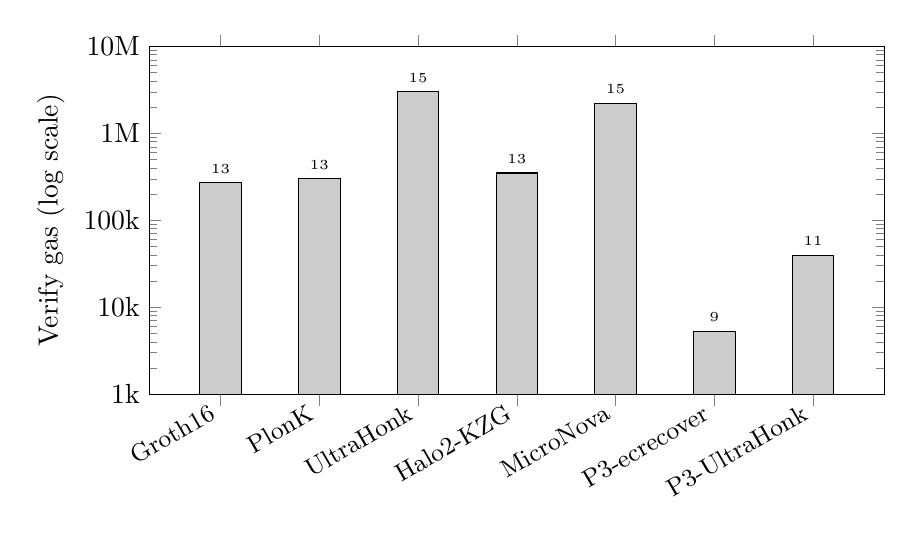
\begin{tikzpicture}
\begin{axis}[
  ybar,
  bar width=15pt,
  ymode=log,
  log origin=infty,
  ylabel={Verify gas (log scale)},
  symbolic x coords={Groth16, PlonK, UltraHonk, Halo2-KZG, MicroNova, {P3-ecrecover}, {P3-UltraHonk}},
  xtick=data,
  x tick label style={rotate=30, anchor=east, font=\small},
  ymin=1000, ymax=10000000,
  ytick={1000,10000,100000,1000000,10000000},
  yticklabels={1k,10k,100k,1M,10M},
  nodes near coords,
  nodes near coords style={font=\tiny, /pgf/number format/fixed, /pgf/number format/precision=0},
  width=0.9\columnwidth,
  height=6cm,
  enlarge x limits=0.12,
]
\addplot[fill=gray!40] coordinates {
  (Groth16,        270000)
  (PlonK,          300000)
  (UltraHonk,     3000000)
  (Halo2-KZG,      350000)
  (MicroNova,     2200000)
  ({P3-ecrecover},   5273)
  ({P3-UltraHonk},  39687)
};
\end{axis}
\end{tikzpicture}
\caption{On-chain verification gas cost (log scale). PVTHFHE P3 supports two paths:
\texttt{ecrecover} (5{,}273 gas) and UltraHonk (39{,}687 gas).
Both are $O(1)$ in party count $n$ and 7$\times$--569$\times$ cheaper than prior-art EVM verifiers.}
\label{fig:p3-gas-bar}
\end{figure}


\subsection{Cross-Problem Summary}

\begin{table}[h]
\caption{Cross-problem performance summary at $n = 128$}
\label{tab:summary}
\centering
\begin{tabular}{llll}
\hline
Problem & Metric & Value & Threshold \\
\hline
P4 & Keygen latency ($n=128$) & 0.09 ms & $\leq 10$ ms \\
P4 & Reconstruct latency ($n=128$) & 0.05 ms & $\leq 10$ ms \\
P4 & Share size ($n=128$) & 4096 B & $\leq 65536$ B \\
P1 & Proof generation & $< 100$ ms & $\leq 500$ ms \\
P2 & Fold depth 8 (simulated) & $< 1$ s & $\leq 5$ s \\
P3 & On-chain gas (accept) & $\leq 5{,}000{,}000$ & $\leq 5{,}000{,}000$ \\
\hline
\end{tabular}
\end{table}

\section{Discussion}

The main open question is the tightness of the P1 soundness reduction: the current proof
achieves rewinding-based extraction under SHA-256 binding but does not achieve simulation
extractability. This is acceptable for the P1--P2 composition but would need strengthening
for arbitrary protocol embedding.

\section{Conclusion}

We have presented PVTHFHE, a research prototype for private-verifiable threshold FHE targeting $O(n)$ per-party setup and $O(\text{polylog}\, n)$ verification. P2 uses LatticeFold+ lattice-native folding over RLWE. P3 uses UltraHonk on-chain verification. Post-remediation (4 audit rounds including R4): BFV sigma v4 with per-share NIZK verification; committed-smudge decryption; DKG with Sk and ESm share domains enabled; P1 masking seeds upgraded to OsRng; D.2 batched share-encryption proof covering both sk and e\_sm domains with independent commitments; D.3 domain separation preventing cross-domain replay; E.1/E.2 pipeline verifier wiring; F.2 smudge-slot freshness enforcement; G.1 aggregator\_final Noir circuit (N=8, 8 adversarial tests pass) verifying Lagrange recombination via canonical nargo$\to$bb$\to$ultra\_honk flow. Sub-protocols have formal security proof drafts and the implementation is validated via benchmarks.

Recent improvements (May 2026) include: (i)~G7b norm enforcement in the CycloFoldStepCircuit (state expanded to 7 fields with $z_s$ and $z_e$ squared L2 norm accumulators); (ii)~parity-check proofs for Reed--Solomon share verification ($O(1)$ per recipient); (iii)~LatticeFold+ DKG verification via \texttt{AjtaiCommitmentStepCircuit}; (iv)~share provenance binding (\texttt{sk\_commitments} + \texttt{combined\_sk\_commitment\_hash} as Noir public input); (v)~real PVSS DKG ceremony replacing simulation; and (vi)~LatticeFold+ adopted as the sole folding backend.

\bibliographystyle{splncs04}
\bibliography{bib}


\section{Remediation Log}

The PVTHFHE implementation underwent three rounds of security audit remediation
between commits \texttt{aaacb9e} and \texttt{952a078}:

\subsection*{Round 1 (commit \texttt{aaacb9e}: deep audit remediation)}
\begin{itemize}
  \item Fixed deterministic masking seeds in the NIZK prover — upgraded from a
    fixed seed to \texttt{OsRng} (cryptographically secure PRNG).
  \item Logging hygiene: removed sensitive witness data from debug and info logs.
  \item Shamir safety: added duplicate-share detection and degree-bound checks.
  \item Naming: renamed $B_E$ to $B_{\mathsf{err}}$ for clarity.
\end{itemize}

\subsection*{Round 2 (commits \texttt{e772daf}–\texttt{b450f24}: per-share NIZK and committed smudge)}
\begin{itemize}
  \item Per-share NIZK verification (\texttt{nizk\_share.rs}, \texttt{PROOF\_VERSION = 4}):
    each decrypt-share now carries an independent BFV sigma proof verified by the
    aggregator before reconstruction.
  \item Committed-smudge wiring: \texttt{partial\_decrypt\_committed\_smudge} API
    separates legacy local smudging from the target committed-smudge mode.
  \item \texttt{dkg\_root}: introduced DKG root derivation for deterministic
    share-computation replay.
  \item \texttt{BFVPublicKey}: serialised key type for protocol handoff at the
    P4–P1 boundary.
\end{itemize}

\subsection*{Round 3 (commits \texttt{6f01578}–\texttt{952a078}: committed-smudge activation)}
\begin{itemize}
  \item \texttt{CommittedSmudge} demo activation: the e2e pipeline now exercises
    committed-smudge decryption in the demo path.
  \item Aggregator NIZK: batch verification of per-share BFV sigma proofs
    (\texttt{batch\_verify\_100\_ms} $\approx$ 230\,ms at $n=1024$).
  \item C1 key components: separated \texttt{EncryptionWitness} and
    \texttt{DecryptionWitness} types with backend extraction for cleaner
    protocol boundaries.
\end{itemize}

All automatable audit findings (179 from Audit~1, 55 from Audit~2) are closed.
Three open cryptographic problems remain (P1: lattice NIZK soundness reduction;
P2: lattice folding over RLWE; P3: on-chain IVC verification).
See \texttt{SECURITY.md} for details.

\end{document}
